\documentclass[Bachelorarbeit.tex]{subfiles}
\begin{document}
\chapter{Konzeption}
\label{chap:entwicklung}
Nachdem im letzten Kapitel die allgemeinen Analysen durchgeführt wurden, soll im Verlauf dieses Kapitels die Planung für den Prototypen abgeschlossen werden.
Für diesen Zweck wird, aufbauend auf den Ergebnissen der bisherigen Kapitel, ein Konzept vorgestellt.\\
\\
Ein weitere wichtiger Bestandteil in diesem Kapitel stellen die \nameref{chap:analyse:sec:interviews} da.
Diese \nameref{chap:analyse:sec:interviews} werden durchgeführt um zu analysieren auf welche Art und Weise  Domänenexpert\_innen arbeiten.
Dadurch soll zum einen herausgefunden werden wo sich aktuell Flaschenhälse, in ihren Workflows befinden und zum anderen, was sie für Wünsche und Anforderungen an ihre Planungswerkzeuge stellen.\\
\\
\begin{comment}

Anschließend wird, auf den Personen aus den \nameref{chap:analyse:sec:interviews} aufbauend eine \nameref{persona} erstellt.
Dies porträtieren eine fiktive Person aus der Zielgruppe und soll als Avatar die Entwicklung unterstützen um den Prototypen möglichst zielgerichtet auszuarbeiten.
\\
\\
Designentwurf
\end{comment}


\section{Interviews}
\label{chap:analyse:sec:interviews}
Dieser Teil beschäftigt sich mit der Fragestellung, wie Personen ihre Außendienstlichen Tätigkeiten organisieren, welchen Herausforderungen sie im beruflichen Alltag gegenüberstehen und welche Verbesserungen sie sich wünschen. 
Für diesen Zweck wurde die Form eines Experteninterviews auf der Basis eines Leitfadens gewählt.
Dabei liegt der Fokus des Interviews auf einem "`Klar definierte Wirklichkeitsausschnitt"' (vgl. \cite{Mayer2006}, S. 36)
Bei diesem Wirklichkeitsausschnitt handelt es sich bei den Interviews um die Expertise der befragten Personen zu dem Prozess der Außendienstplanung.
Bei den befragten Personen handelt es sich bei allen Interviews um Firmenkontakte des Unternehmens Perfany.
Da die Identität der befragten Personen sowie die Unternehmen für die sie tätig sind keinen direkten Einfluss auf die Ergebnisse haben, werden die entsprechenden Informationen nur umschrieben und nicht explizit genannt.\\
\\
Das Ziel dieser Interviews besteht darin, ein besseres Gefühl für den Ist-Zustand zu bekommen und Anhand dieser Erkenntnisse die möglichen Defizite zu analysieren.
Des weiteren bietet der Ansatz die Möglichkeit, Verbesserungswünsche und Ideen von Personen aus der Domäne zu erhalten, ohne dass sie zuvor durch den Blick aus der Entwicklungssicht verfälscht wurden.


\subsection{Ausarbeitung des Leitfadens}

Als erster Schritt soll ein Leitfaden für die Interviews definiert werden. 
Dieser soll zum einen als Gedankenstütze für die Interviews dienen und zum anderen in Form eines roter Fadens zu einem strukturierten Ablauf führen.
Das Ziel der Interviews liegt darin, ein besseres Verständnis zu erlangen, wie die einzelnen Personen arbeiten und mit welchen Mitteln.
Diese Informationen bilden eine wichtige Grundlage, um bestehende Probleme und Stolpersteine im aktuellen Workflow zu identifizieren und bei der Realisierung des Prototypen zu vermeiden. 
Des Weiteren bilden die Interviews einen wichtigen Einblick in die Domäne, anhand derer eine nutzer\_innenzentrierte Lösung so nah wie möglich an der Realität entwickelt werden soll.\\
\\
Grundsätzlich sollten allgemeine Informationen zum Interview festgehalten werden, wie die Dauer und das Datum des Interviews.
Bezüglich der Person sind die Tätigkeit im Unternehmen, die Verantwortung bei der Planung und die Art der Beschäftigung (angestellt oder selbstständig) interessant.
Des Weiteren spielt die Größe, das Betätigungsfeld und das Einzugsgebiet des Unternehmens eine Rolle für die Befragung.
Um eine bessere Strukturierung der Informationen zu erhalten, wird zu erst der Standardablauf erfragt. 
Anschließend wird geklärt, welche Sonderfälle auftreten können und wie diese jeweils gehandhabt werden.
Den Abschluss der Befragung bildet eine Selbstbeurteilung des Workflows. 
Dieser ist zum einen in Probleme und zum anderen in Wünsche unterteilt.
Bei dem ersten Punkt wird explizit nachgefragt, welche Probleme oder Engstellen die Probanden im Alltag festgestellt haben, während beim zweiten Punkt nach den Wünschen beziehungsweise sinnvollen Ergänzungen gefragt wird die sie sich selbst überlegt haben. 
Dabei sind alle Fragestellungen in den Interviews als offene Fragen formuliert. 
Dies hat den Vorteil, dass die befragten Personen zum einen nicht eingeschränkt werden und zum anderen ausführlich und detailliert Antworten können (vgl. \cite{Mayer2006}, S. 36).
Die finale Version des Leitfadens kann im Anhang eingesehen werden (\nameref{anhang:leitfaden_interviews}). 







\section{Ergebnisse der Interviews}
Bei den Personen handelt es sich um drei verschiedene Individuen die in drei verschiedenen Berufen in drei verschiedenen Firmen arbeiten und für ihren Alltag die unterschiedlichsten Systeme und Medien verwenden. 
Dabei sind alle befragten Personen seit mindestens zwei Jahren in ihrer Funktion tätig und sind für die Planung ihrer Routen selbst verantwortlich.
\\
\\
Für eine bessere Übersicht ist die Ausarbeitung der Ergebnisse in die drei Gruppen
\nameref{UebersichtDerInterviews}, \nameref{subsubsec:Ergebnisse der Interviews:gemeinsamkeiten} und \nameref{AnalyseInterviews} unterteilt. 


\subsection{Übersicht der Interviews}
\label{UebersichtDerInterviews}
Das Ziel dieses Abschnitts liegt darin, einen Überblick über die einzelnen Interviews zu geben. 
Für diesen Zweck wurde für jedes Interview eine kurze Zusammenfassung über den Ablauf des Workflows, wie er geschildert wurde, zusammengestellt.

\paragraph*{Übersicht - \nameref{anhang:interview1}} 

Die Person arbeitet für einen nationalen Konzern im Bereich Dienstleistung in der Arbeitskräftevermittlung. 
Der Einzugsbereich umfasst ausschließlich das Land Vorarlberg, Österreich.
Während die Kontaktdaten über das hauseigene \ac{ERP} gepflegt und gesucht werden, wird die Terminplanung und -Verwaltung größtenteils mithilfe eines Taschenkalenders abgewickelt.
Dabei wird im voraus für jede Kalenderwoche eine Region definiert. 
Für die gewählte Kalenderwoche werden mit Kunden in der entsprechenden Region Termine vereinbart.\\


\paragraph*{Übersicht - \nameref{anhang:interview2}}
Bei dem zweiten Interview handelt es sich um eine Person die für die Leitung der Firma sowie den Außendienst verantwortlich ist.
Der Tätigkeitsbereich des \ac{KMU}, mit Firmensitz in Wien, bezieht sich auf den Vertrieb von Hifi-Geräten für den professionellen Einsatz in Tonstudios.
Neben Österreich und dem EU-Raum gehört auch Russland zu dem Zuständigkeitsbereich des Unternehmens.
Dabei werden Außendienstrouten nach Bedarf geplant.
Für diesen Zweck wird im ersten Schritt eine Route definiert. 
Anschließend werden, auf Basis der Route, die relevanten Bezirke gesucht.
Anhand einer Postleitzahlenkarte werden in mehreren Schritten die Postleitzahlen analysiert, welche auf der Route liegen.
Diese Postleitzahlen dienen als Kriterium für den Filtervorgang im Kundenverzeichnis auf Basis dessen schlussendlich die Kunden ausgesucht werden.

\paragraph*{Übersicht - \nameref{anhang:interview3}}
Bei dem letzten Interview handelt es sich um eine Person, welche eine Anstellung in den Bereichen des Key Account Management sowie Projektleitung in einem \ac{KMU} inne hat.
Bei dem Unternehmen selbst handelt es sich um eine Werbeagentur mit dem Hauptsitz in Vorarlberg sowie einer Niederlassung in der Schweiz.
Der Tätigkeitsschwerpunkt der Firma liegt im Dreiländereck am Bodensee\footnote{Uferbereich und nahes Umland am Bodensee der Länder Österreich, Deutschland und Schweiz}. 
Die befragte Person plant die Touren nach Bedarf in eigener Verantwortung.
Wenn bei einem Kunden Bedarf für einen Termin besteht, wird grob analysiert, welcher Kunde auf dem Weg noch relevant wäre für einen Termin.

\subsection{Gemeinsamkeiten}
\label{subsubsec:Ergebnisse der Interviews:gemeinsamkeiten}
Abstrakt gesprochen unterscheiden sich die Workflows in ihren Grundzügen nicht deutlich von einander (siehe Abb.: \ref{fig:abstrakterWorkflowPlannung}). 
Es besteht eine Grundmenge von Daten (beispielsweise Kunden\_innen oder Stammdaten). 
Aus dieser Grundmenge wird mit Hilfe von Filterungs- und/oder Anreicherungsschritten die Teilmenge der relevanten Daten gebildet, was wiederum beliebig oft wiederholt wird (jeweils für jedes Entscheidungskriterium).
Nachdem die Teilmenge der relevanten Daten den Anforderungen des Szenarios entspricht, wird mit der Auswahl der einzelnen Elemente fortgefahren.
Die Menge dieser gewählten Elemente bilden schlussendlich die getroffene Auswahl für die Planung.\\
\\
Bei dieser Schilderung handelt es sich nur um den kleinsten gemeinsamen Nenner der geführten Interviews.
Die Unterschiede liegen dabei in den Details, wie beispielsweise die Auswahl für die Teilmenge der relevanten Daten gebildet wird.
Speziell die Probleme, die in den jeweiligen Details auftreten, werden im folgenden Abschnitt genauer erläutert.

\begin{figure}[h]
	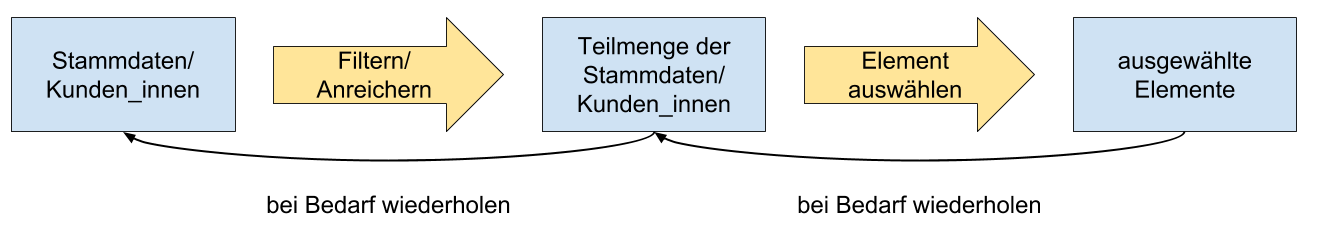
\includegraphics[width=\linewidth]{img/analyse/abstrakterWorkflowPlannung}
	\caption[abstrakter Planungsworkflow]{abstraktes Model des Planungsworkflows (Quelle: eigene Ausarbeitung)}
	\label{fig:abstrakterWorkflowPlannung}
\end{figure}

Mithilfe der Interviews wurden zwei weitere Phasen identifiziert, welche für die Praxis von hoher Relevanz sind und im vorhergehenden Kapitel noch nicht beachtet wurden.
Dabei handelt es sich zum einen um die Unterstützung während der Durchführung der Außendiensttätigkeit und zum anderen um die Aufbereitung der Daten nach der Außendiensttätigkeit.

\subsection{Analyse}
\label{AnalyseInterviews}
Alle in den \nameref{chap:analyse:sec:interviews} besprochenen Workflows haben an gewissen Stellen Verbesserungspotential. 
Um die Erkenntnisse aus den Interviews bestmöglich zu nutzen, müssen die vorhandenen Informationen in eine auswertbare Form gebracht werden.
Für diesen Zweck wurde eine Sammlung von Kategorien definiert, die im folgenden Abschnitt genauer erklärt werden (siehe Abschnitt \nameref{analyse:kategorien}).
Anhand der genannten Probleme und Wünsche (beziehungsweise die Ursachen der Wünsche) wurde separat für jedes Interview eine eigene Gewichtung der betreffenden Kategorien durchgeführt (siehe Abschnitt \nameref{analyse:gewichtung}). 
Auf Basis der Erkenntnisse aus dieser Analyse soll schlussendlich im Abschnitt \nameref{chap:entwicklung:sec:konzept} das Konzept für den Prototypen entstehen.


\subsubsection{Kategorien}
\label{analyse:kategorien}
In folgenden Abschnitten werden die einzelnen Kategorien aufgezeigt und die Idee dahinter verdeutlicht.
Die Reihenfolge der Kategorien soll keine Wertung darstellen.

\paragraph{Systembruch}
\label{interviewsAnalyseSystembruch}
Damit ist gemeint, dass parallel zum bestehenden System zusätzliche Drittsoftware oder gar andere Medien eingesetzt werden.
Dies ist laut den geführten Interviews auf den Grund zurückzuführen, dass das bestehende System entweder nicht über die benötigte Funktionalität verfügt
\footnote{
	Diese Meinung stammt aus der Sicht des Personals. 
	Ein weiteres denkbares Szenario ist, dass die Funktionalität zwar gegeben ist, allerdings das Personal nicht darüber informiert beziehungsweise geschult wurde.
	} 
oder nur umständlich/aufwendig zu bedienen ist.
Dabei können solche Systembrüche zu diversen Problemen führen. 
Mögliche Probleme können im Datenschutz
\footnote{
	Beispielsweise Weitergabe von Kunden/Patientendaten an Dritte.
	}
	, der unautorisierten Weitergabe von Firmengeheimnissen oder schlichtweg in Brüchen des Informationsmanagements liegen.  
Bei den durchgeführten Interviews wurden folgende drei Szenarien mit Systembrüchen identifiziert:


\paragraph{Systembruch: Termine und Kalender}
Aufgrund der fehlenden Funktionalität Termine im bestehenden System verwalten zu können wird in \nameref{anhang:interview1} beschrieben, dass die Terminplanung mithilfe eines Taschenkalenders bewältigt wird. 
In \nameref{anhang:interview3} wird eine Kombination aus einem privaten Kalender in Microsoft Outlook und einem Taschenkalender verwendet. 
Bei beiden Interviews besteht das Problem, dass die Termine nicht für Dritte (Beispiel: Urlaubsvertretungen, etc.) einsichtig sind.

\paragraph{Systembruch: Routenberechnung}
Um eine Routenberechnung zu den ausgewählten Partnerunternehmen zu optimieren, wird laut \nameref{anhang:interview2} und \nameref{anhang:interview3} regelmäßig auf Google Maps zurückgegriffen. 
Für diesen Zweck müssen die Kontaktdaten entweder umständlich kopiert oder von Hand übertragen werden.


\paragraph{Systembruch: Export der Daten für den Außendienst}

Ein weiterer Punkt für die Verwendung von Drittsoftware liegt in der Aufbereitung der Informationen für den Außendienst.
Nachdem eine Route geplant wurde, müssen wichtige Informationen, wie beispielsweise Verkaufzahlen und Ähnliches auf Papier vorliegen. 
Für diesen Zweck werden entweder, wie in \nameref{anhang:interview2} genannt, die wichtigsten Informationen auf Post It`s übertragen, oder, wie in \nameref{anhang:interview3} beschrieben, von Hand mittels Eopieren und Einfügen in ein Textverarbeitungsprogramme übertragen und anschließend gedruckt.
\\ [1.0cm]

\paragraph{Datenstrukturen}
\label{interviewsAnalyseDatenstrukturen}
Während im letzten Abschnitt auf die bestehenden Systembrüche eingegangen wurde, liegt der Schwerpunkt hier auf den unzureichenden Datenstrukturen und weniger auf der Funktionalität der bestehenden Systeme. 
Dabei ist zu berücksichtigen, dass die richtige Datenstruktur eine Grundlage für die Implementierung von Funktionalitäten darstellt. 
Bei der Analyse der Interviews sind dabei folgende Nennungen hervorgetreten:

\paragraph{Datenstrukturen: Termine}
Sowohl in \nameref{anhang:interview1} als auch in \nameref{anhang:interview3} ist es möglich, Termine beziehungsweise Daten im System zu hinterlegen. 
Allerdings handelt es sich bei den Datumsfeldern bei beiden Systemen ausschließlich um Textfelder. 
Das bedeutet, dass man zwar das Datum angeben kann, allerdings das System sehr eingeschränkt ist bei der Interaktion mit diesen Werten. 
Somit lassen sich zum Beispiel keine wiederkehrende Termine erstellen (siehe \nameref{anhang:interview3}).


\paragraph{Datenstrukturen: Kundenspezifische Meta-Daten}
Der letzte Punkt behandelt die fehlenden Datenstrukturen von kundenspezifischen Meta-Daten.
Dieser Begriff wurde im Zuge der Interviews vom Autor geprägt und bezeichnet Daten und Informationen über Kunden, die nicht zu den klassischen Firmendaten, wie beispielsweise Umsatzzahlen zählen. 
Vielmehr haben diese Informationen den Charakter von firmeninternen Notizen, wie sie auch in den meisten Systemen aktuell gehandhabt werden.
Ein Beispiel für diese Daten wären zum Beispiel die persönlichen Interessen/Abneigungen, Smalltalk-Themen und produktiv Zeiten\footnote{Beispiel: ...ist Frühaufsteher, ...Abschlüsse lassen sich am besten am Abend machen, etc.} der Kunden\_innen. 
Wie in \nameref{anhang:interview2} und \nameref{anhang:interview3} festgestellt wurde, sind diese Daten für die Personen in der Planung ein hilfreiches Werkzeug. 
Leider ist im besten Fall bei Kundenkontakten ein allgemeines Notizfeld vorgesehen. 
Ähnlich wie bei den Terminen ist es schwierig diese Daten sinnvoll zu verwenden, solange sie nur als reiner Text vorliegen.
\\ [1.0cm]

\paragraph{Routenverwaltung}
\label{interviewsAnalyseRoutenverwaltung}
Das Endprodukt einer Außendienstplanung stellt eine fertig gestellte Route dar,  mit allen Daten und Informationen die der Außendienstmitarbeiter für die Durchführung benötigt.
Leider ist in keinen der durchgeführten Interviews aktuell eine solche Funktion gegeben oder angedacht.
Im Moment werden Aspekte der Routenverwaltung bei allen drei Interviews angegeben.
Dabei handelt es sich um die Erstellung, die Bearbeitung und das Exportieren für den Außendiensteinsatz (siehe \nameref{anhang:interview1}, \nameref{anhang:interview2} und \nameref{anhang:interview3}). 
\\ [1.0cm]

\paragraph{Filterungsverfahren}
\label{interviewsAnalyseFilterungsverfahren}
Den ersten Schritt der Planung stellt das Filtern nach relevanten Datensätzen dar.
Aktuell geschieht dies im besten Fall durch das Definieren von verschiedenen Filtereinstellungen (Beispielsweise in pery).
Umständlich wird es, wenn die benötigten Daten auf verschiedenen, nicht mit einander verbundenen Systemen verteilt sind (siehe Abschnitt \nameref{interviewsAnalyseSystembruch}). 
Diese Verteilung hat in der Praxis zur Folge, dass Zwischenergebnisse notiert und händisch miteinander verglichen werden müssen.
Was wiederum zum einen umständlich und zum anderen fehleranfällig ist, in Hinsicht darauf, dass Daten übersehen werden könnten (siehe \nameref{anhang:interview2} und \nameref{anhang:interview3}).
\\ [1.0cm]

\paragraph*{Übersicht Standorte}
\label{interviewsAnalyseStandorte}
Bei allen Workflows spielt der Standort der einzelnen Kunden eine entscheidende Rolle bei der Planung.
In den meisten Systemen ist bei jedem Kontakt eine Adresse hinterlegt welche in Form einer Textausgabe angezeigt wird.
Da in allen drei Interviews die fehlende Übersicht der jeweiligen Standorte am häufigsten angegeben wurde, sollte man die Ursachen genauer betrachten. 
Die Nennungen wurden dabei in folgende zwei Kategorien eingeteilt:

\paragraph{Übersicht Standorte: in der Planung}
\label{UebersichtStandortePlanung}
Nach der Filterung der Datensätze werden die Informationen meist in Tabellenform angezeigt.
Dabei ist jeder Kunde inklusive seiner Adresse in einer Zeile aufgeführt.
Bei keinen der Interviews wurde angegeben, dass außer der Adresse weitere geografische Informationen, wie beispielsweise Distanzen oder ähnliches, verfügbar sind.
Der einzige Weg eine Reihung durchzuführen basiert entweder auf der Postleitzahl
\footnote{
	numerisch auf- beziehungsweise absteigend
	} 
(siehe \nameref{anhang:interview2}) oder auf dem Namen der Stadt
\footnote{
	alphabetisch auf- beziehungsweise absteigend
	}. 
Allerdings ist der Mehrwert einer Reihung oder Filterung nach harten Grenzen (Postleitzahlen oder Stadtnamen) oft nicht zielführend, da der geografische Kontext verloren geht.
Dies wird an folgenden Beispiel deutlicher (siehe Abb.: \ref{fig:HarteGrenzen}). 
Angenommen es gibt zwei Kunden\_innen die eine Distanz von knapp 300 Metern trennt. 
Da sie beide durch eine Stadtgrenze getrennt sind, werden sie bei der Sortierung an unterschiedlichen Stellen aufgelistet.
Dabei gehen relevante Informationen wie zum Beispiel ein Standort der 300 Meter in der nächsten Stadt liegt schlichtweg verloren (siehe \nameref{anhang:interview1} und \nameref{anhang:interview2}). 
 
\begin{figure}[h]
\centering
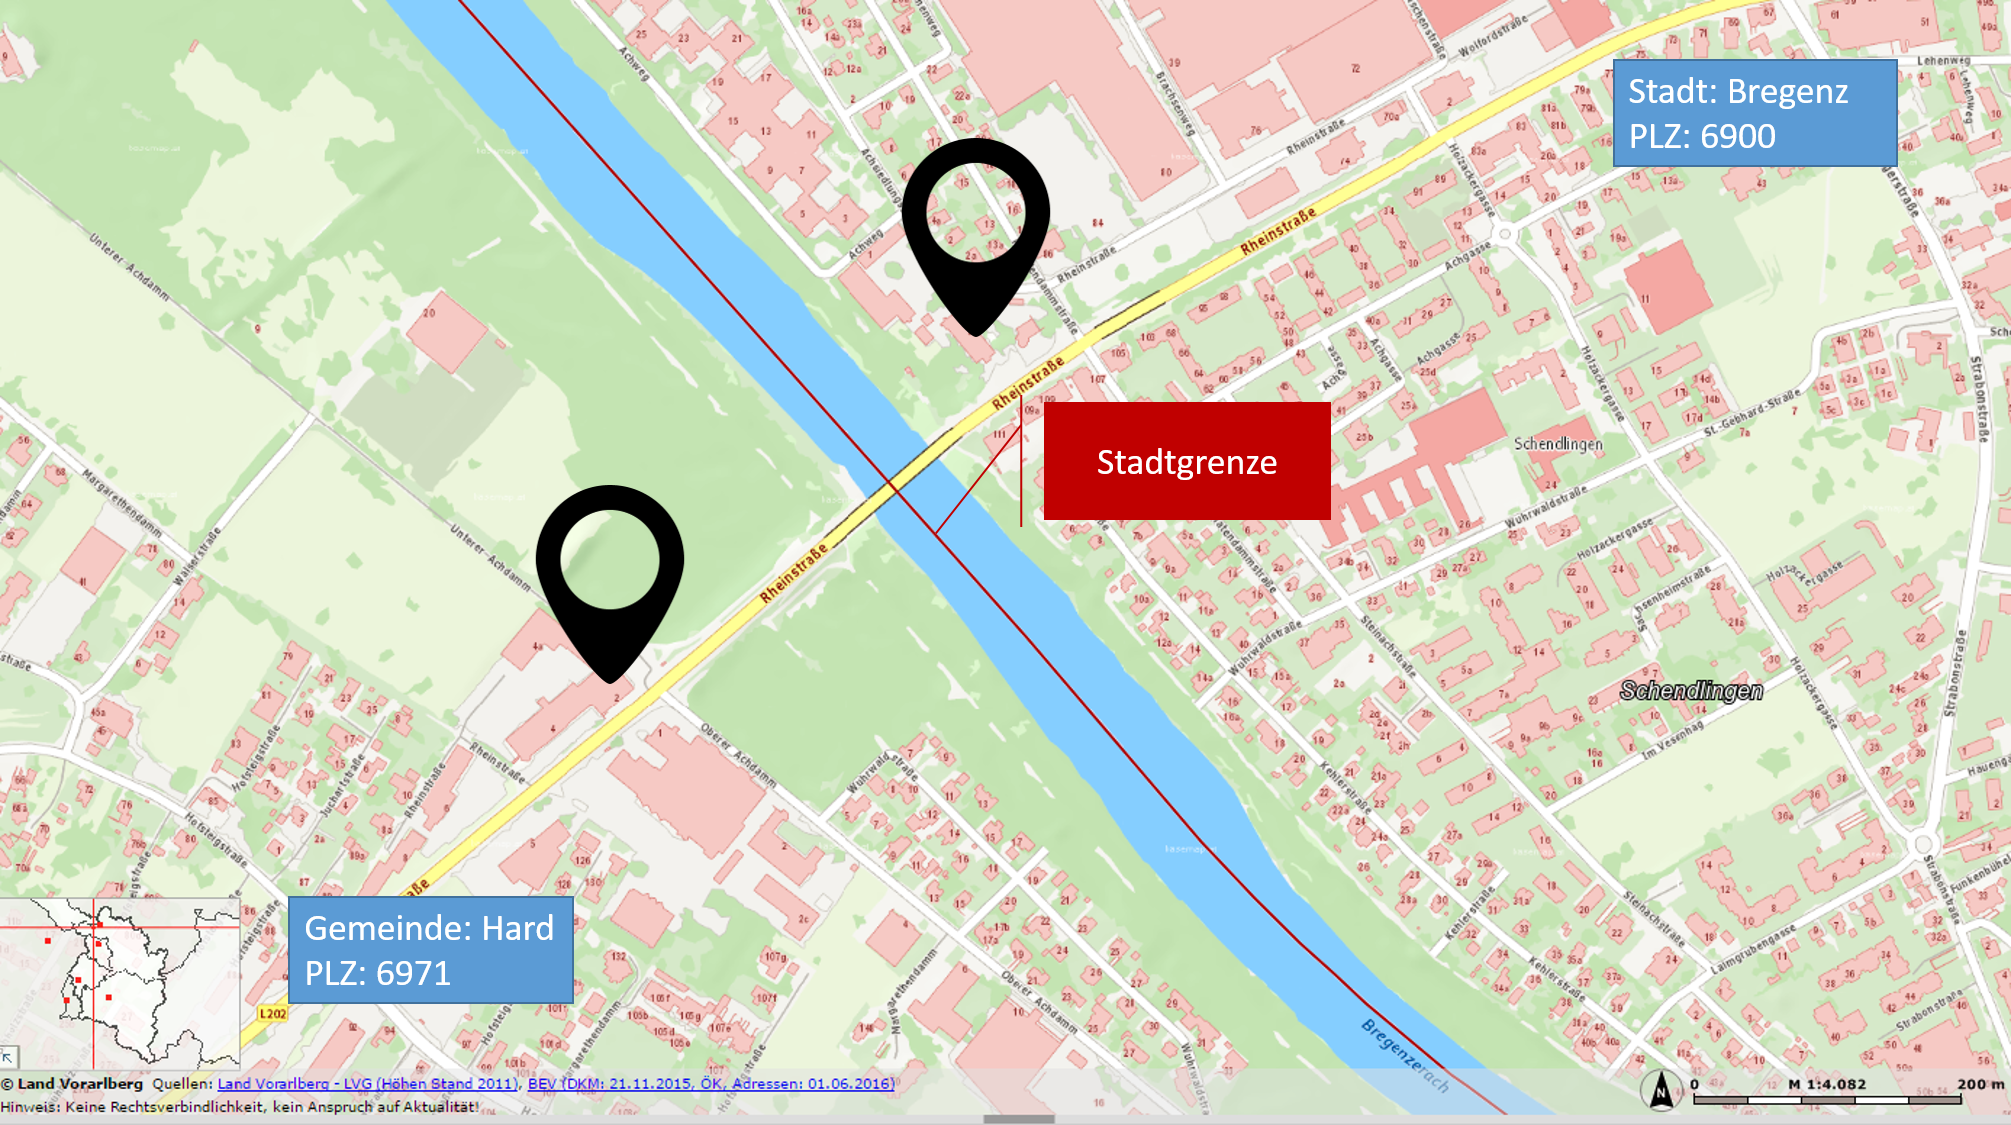
\includegraphics[width=1\linewidth]{img/Interviews/HarteGrenzen}
\caption[Probleme mit harten Grenzen]{Problem bei der Filterung oder Sortierung auf Basis von Ortsgrenzen und/oder Postleitzahlen (Quelle: eigene Ausarbeitung | Daten und Kartenmaterial: http://vogis.cnv.at/)}
\label{fig:HarteGrenzen}
\end{figure}

Die Grenze der zumutbaren Übersicht wird erreicht, wenn geografische Informationen mit weiteren Faktoren, wie Kundendaten, in Kontext gesetzt werden sollen. 
Dies wird aktuell in einzelnen Zwischenschritten\footnote{Dabei ist die Anzahl der Zwischenschritte von der Anzahl der benötigten Faktoren abhängig} gelöst und ist dadurch zum einen fehleranfällig und zum anderen zeitaufwendig (siehe \nameref{anhang:interview2}).

\paragraph{Übersicht Standorte: in der Durchführung}
Ähnlich wie bei der Planung wurden auch bei der Durchführung des Außendiensteinsatzes Defizite bei der Übersichtlichkeit der Standorte festgestellt. 
Dies tritt vor allem dann auf, wenn auf Grund von Änderungen spontan reagiert werden muss.
Dies sind meistens Einschübe oder Änderungen von Termin während des Einsatzes (siehe \nameref{anhang:interview2}). 
In solchen Fällen muss zügig ein Ersatz (alternativer Termin) gefunden werden, wofür sich meist Kunden in der Nähe (aktuelle Position des Personals) anbieten (siehe \nameref{anhang:interview2}).
In den Interviews wurde besprochen, dass für diesen Zweck meist mögliche Alternativen im Vorfeld vorbereitet und meist in ausgedruckter Form mitgeführt werden. 
\newpage

\subsubsection{Gewichtung der Kategorien}
\label{analyse:gewichtung}

Nachdem die verschiedenen Kategorien definiert sind, werden die Probleme und Wünsche der einzelnen Interviews Kategorien\footnote{
	Siehe Abschnitt \nameref{analyse:kategorien} für weitere Informationen.
	}
zugeteilt.
Dabei ist es auch möglich, dass ein Problem/Wunsch mehreren Kategorien zugeteilt werden kann.
Anhand der Nennungen in den Interviews wird für jede Kategorie eine eigene Gewichtung vorgenommen.
Die Werte der Gewichtung erstrecken sich dabei über einen ganzzahligen Wertebereich von null bis vier, wobei der Wert vier die meisten Nennungen erhalten hat\footnote
{Der Wertebereich von null bis vier wurde vom Autor festgelegt}.

\subsubsection{Präsentation der Ergebnisse}
Zum verständlichen Präsentieren der Ergebnisse dienen folgende zwei Grafiken.\footnote
	{siehe Abb.: \ref{fig:KategorienGesamt} und Abb.: \ref{fig:GewichtungNachInterview}}
Zum einen wurden die Daten nach Kategorien gruppiert (siehe Abb.: \ref{fig:KategorienGesamt}),
zum anderen wurden die Daten nach Interviews gruppiert (siehe Abb.: \ref{fig:GewichtungNachInterview} - \nameref{fig:GewichtungNachInterview}).

\begin{figure}[H]
	\centering
	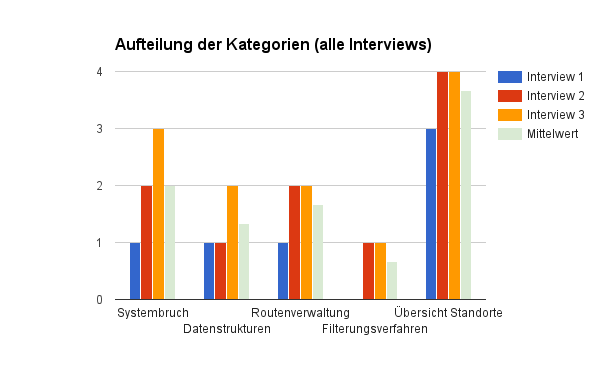
\includegraphics[width=0.9\linewidth]{img/Interviews/KategorienGesamt}
	\caption[Gewichtung der Kategorien (alle Interviews)]{Gewichtung der Kategorien (alle Interviews). Quelle: eigene Ausarbeitung}
	\label{fig:KategorienGesamt}
\end{figure}

\begin{figure}[H]
	\centering
	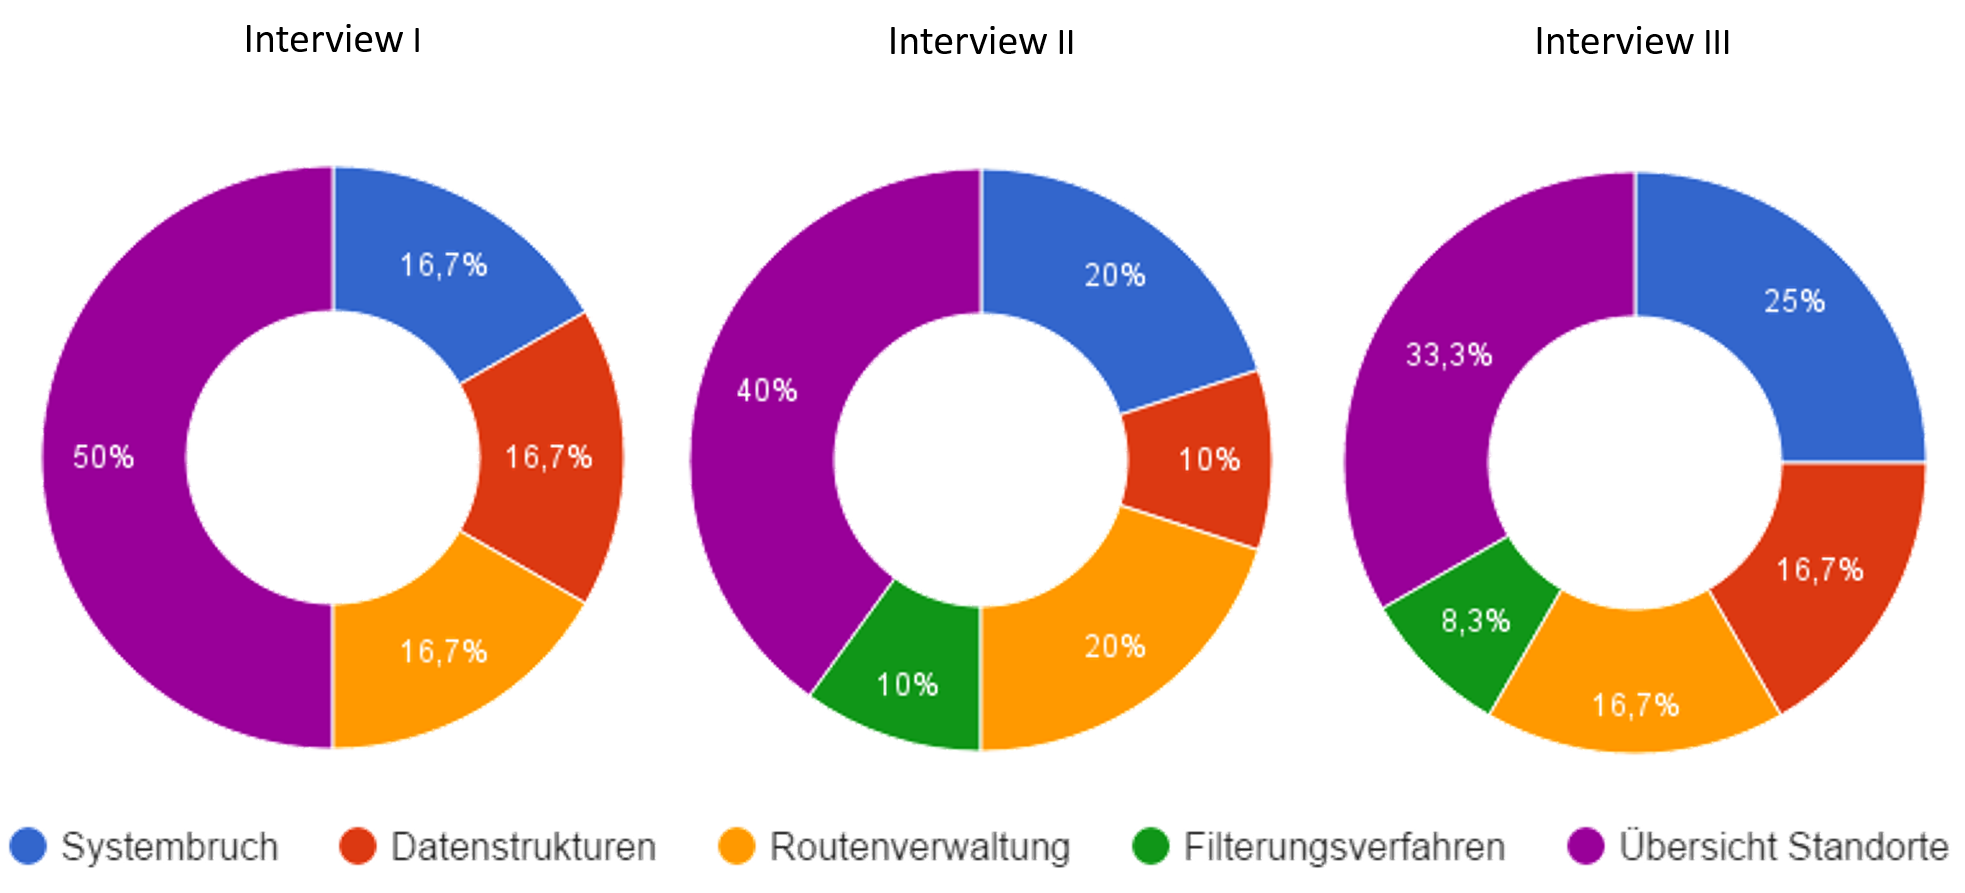
\includegraphics[width=0.9\linewidth]{img/Interviews/VerteilungNachInterview}
	\caption[Relative Gewichtung der Kategorien in den einzelnen Interviews]{Relative Gewichtung der Kategorien in den einzelnen Interviews. Quelle: eigene Ausarbeitung.}
	\label{fig:GewichtungNachInterview}
\end{figure}

Wenn man die Mittelwerte der Kategorien anhand aller Interviews vergleicht (siehe Abb.: \ref{fig:KategorienGesamt}), stellt sich heraus, dass die Kategorie Übersicht Standorte am meisten diskutiert wurde. 
Anschließend folgen die Kategorien Systembruch, Routenverwaltung und Datenstruktur.
Die am wenigsten diskutierte Kategorie ist das Filterungsverfahren. 
Dies ist die einzige Kategorie, welche nicht in allen Interviews diskutiert wurde.
Somit ergibt sich folgende Reihung:

\begin{enumerate}
	\item Übersicht Standorte
	\item Systembruch
	\item Routenverwaltung
	\item Datenstruktur
	\item Filterungsverfahren
\end{enumerate}

Auf die Auswertung folgend wird im kommenden Abschnitt \nameref{chap:entwicklung:sec:konzept} die Planung für den Prototypen erstellt.
Dabei bildet die vorliegende Auswertung, neben den Ergebnissen aus Kapitel \ref{chap:analyse} - \nameref{chap:analyse}, einen Grundstein für die Ausarbeitung.

\newpage

\section{Konzept}
\label{chap:entwicklung:sec:konzept}
Das Ziel dieses Abschnittes besteht darin ein Konzept für die erste Version des Prototypen zu entwickeln mit dem Fokus auf das definierte Szenario der Außendienstplanung. 
Dabei ist zu beachten das anhand der ersten Implementierung des Prototypen evaluiert werden soll ob und in wie fern die zu Grunde liegende \nameref{chap:einfuehrung:sec:idee} dieser Arbeit einen Mehrwert für die Anwender\_innen bietet.
Aus diesem Grund wurde die Entscheidung gefällt, nicht alle Kategorien aus der vorangegangen Analyse zu realisieren.
Dabei soll der Prototyp als Grundlage zwischen dem bestehenden System (Pery) und den ausgewählten Kategorien entwickelt werden, welcher in späteren Implementierungszyklen fortlaufend erweitert werden soll.
Auf Basis der \nameref{AnalyseInterviews}, des vorangegangen Abschnittes, wird an dieser Stelle das Grundlegende Konzept, welches für die erste Implementierung des Prototypen ausgewählt wurde, definiert. \\
\\
Es soll Grundsätzlich möglich sein, unterschiedliche Listen mit ausgewählten Unternehmen (Trips) im System zu erfassen und diese zu bearbeiten (siehe \nameref{anhang:interview1}).
Dabei ist der Funktionsumfang der Liste, im ersten Schritt, auf das Hinzufügen und Löschen von Unternehmen zu der Liste sowie das Erstellen, Umbenennen und Löschen der Liste selbst limitiert.\\
\\
Das Problem des Systembruchs (siehe Abschnitt \nameref{interviewsAnalyseSystembruch}) soll mit durch die Implementierung des Prototyps in Pery gelöst werden. 
Dadurch sind die grundlegenden Informationen zu den Unternehmen schon in Pery über seine \ac{ERP}/\ac{CRM} Funktionalität abgedeckt. 
Zusätzliche Daten die für die Visualisierung notwendig sind, wie Beispielsweise Zeitpunkt des letzten Besuches, werden im Zuge der Implementierung, entweder nachgezogen oder miteinander verknüpft.
Durch diesen Schritt soll sichergestellt werden das alle notwendigen Informationen in Pery abrufbar sind und somit kein Wechsel zwischen verschiedenen Systemen notwendig ist.\\
\\
Ein weiterer oft genannter Punkt der Analyse ist die Übersicht der Standorte von  Unternehmen. 
Dabei sollen die Unternehmensdaten sowohl auf einer Karte als auch klassisch in einer Liste dargestellt werden. 
Es handelt sich bei den verschiedenen Ansichten immer um die gleichen Informationen welche jedoch unterschiedlich visualisiert werden.
Dabei ist besonderes darauf zu achten das der Wechsel zwischen den Ansichten reibungslos abläuft und keinen nennenswerten Mehraufwand darstellt.
Das hinzufügen von Unternehmen zur aktiven Tripliste soll dabei, auf eine ähnliche Vorgehensweise, von beiden Ansichten möglich sein. 
Mithilfe dieser Schrittes können die Anwender\_innen selbst entscheiden welche Ansicht das beste Werkzeug darstellt um ihre Anforderungen zu meistern.


\section{Design-Entwurf}
\label{chap:entwicklung:sec:design_entwurf}

\subsection{Ziele der Gestaltung}
\label{chap:entwicklung:sec:design_entwurf:subs:ziele_der_gestaltung}

\subsubsection*{Ziel: Übersichtlichkeit}
\label{subsub:ziel_uebersichtlichkeit}
Um die Übersichtlichkeit des Prototypen zu steigern ist eine klare und aufgeräumte Oberfläche notwendig. 
Aus diesem Grund müssen die Inhalte, unter der Berücksichtigung der Arbeitsabläufe, in sinnvolle und logische Gruppen aufgeteilt werden. 
Zusätzlich wird darauf wert gelegt markante Elemente wie Farben oder fettgedruckten Text dezent einzusetzen. 


\subsubsection*{Ziel: Vertraute Umgebung}
\label{subsub:ziel_vertraute_umgebung}
Durch das gestalten einer, für die Anwender\_innen, vertrauten Umgebung soll der Wiedererkennungswert von erlernten Verhalten maximiert und die Einarbeitungszeiten minimiert werden.
Dabei sollen die Anwender\_innen das Bewusstsein entwickeln, dass sie das Programm in jeder Situation kontrollieren sowie das mögliche Fehler leicht zu korrigieren sind.



\subsection{Mock-Up - Prototyp Entwicklung}
\label{chap:entwicklung:sec:design_entwurf:sub:mockUps}
Auf Basis des Konzeptes und unter der Berücksichtigung der zuvor definierten Gestaltungsziele soll an dieser Stelle ein erster Entwurf für den Prototyp aufgezeigt werden.\\
\\
Grundsätzlich ist der Prototyp, ähnlich wie die zuvor betrachteten Webservices Google Maps und Airbnb, in drei Bereiche aufgeteilt welche jeweils ein eigenständigen Aufgabenspektrum abdecken. (siehe Abb.: \ref{fig:prototypMockup}). 
Die Entscheidung sich an den bekannten Webservices zu orientieren ist bewusst gefällt wurden um den Anwender\_innen den Eindruck einer bekannten Umgebung zu vermitteln.\\
\\
Im oberen Bereich befindet sich der Kopfbereich des Prototypen (siehe Abb.: \ref{fig:prototypMockup} - Markierung 1). 
Dieser Bereich dient zum einen als Orientierungshilfe in dem er die Anwender\_innen informiert welche Funktionalität des Prototypen sie aktuell verwenden.\footnote{Im diesem Fall ist das die Funktionalität Edit Trip.}
Desweiteren besteht die Möglichkeit in diesem Bereich zwischen den verschiedenen Ansichten (Karten- und Listenansicht) umzuschalten.\\
\\
Der linke Bereich wurde für die Darstellung der Ergebnisse reserviert (siehe Abb.: \ref{fig:prototypMockup} - Markierung 2). 
Hier befinden sich alle Unternehmen, jedes als einzelnes Element, welche zuvor in der Karten- oder Listen Ansicht ausgewählt wurden.
Dabei ist anzumerken das dieser Bereich, unabhängig von dem Wechseln zwischen den verschieden Ansichten, immer angezeigt wird. \\
\\
Im rechten Bereich ist der Platz für den Container mit den austauschbaren Darstellungen reserviert (siehe Abb.: \ref{fig:prototypMockup} - Markierung 3). 
An dieser Stelle wird, je nach Auswahl, die Karten- oder Listenansicht angezeigt.
Dabei werden, an dieser Stelle, immer die gleichen Daten allerdings auf unterschiedliche Weise dargestellt.
Unabhängig von der ausgewählten Ansicht lassen sich die ausgewählten Unternehmen zur Trip Liste (linker Bereich) hinzufügen.

\begin{figure}[h]
\centering
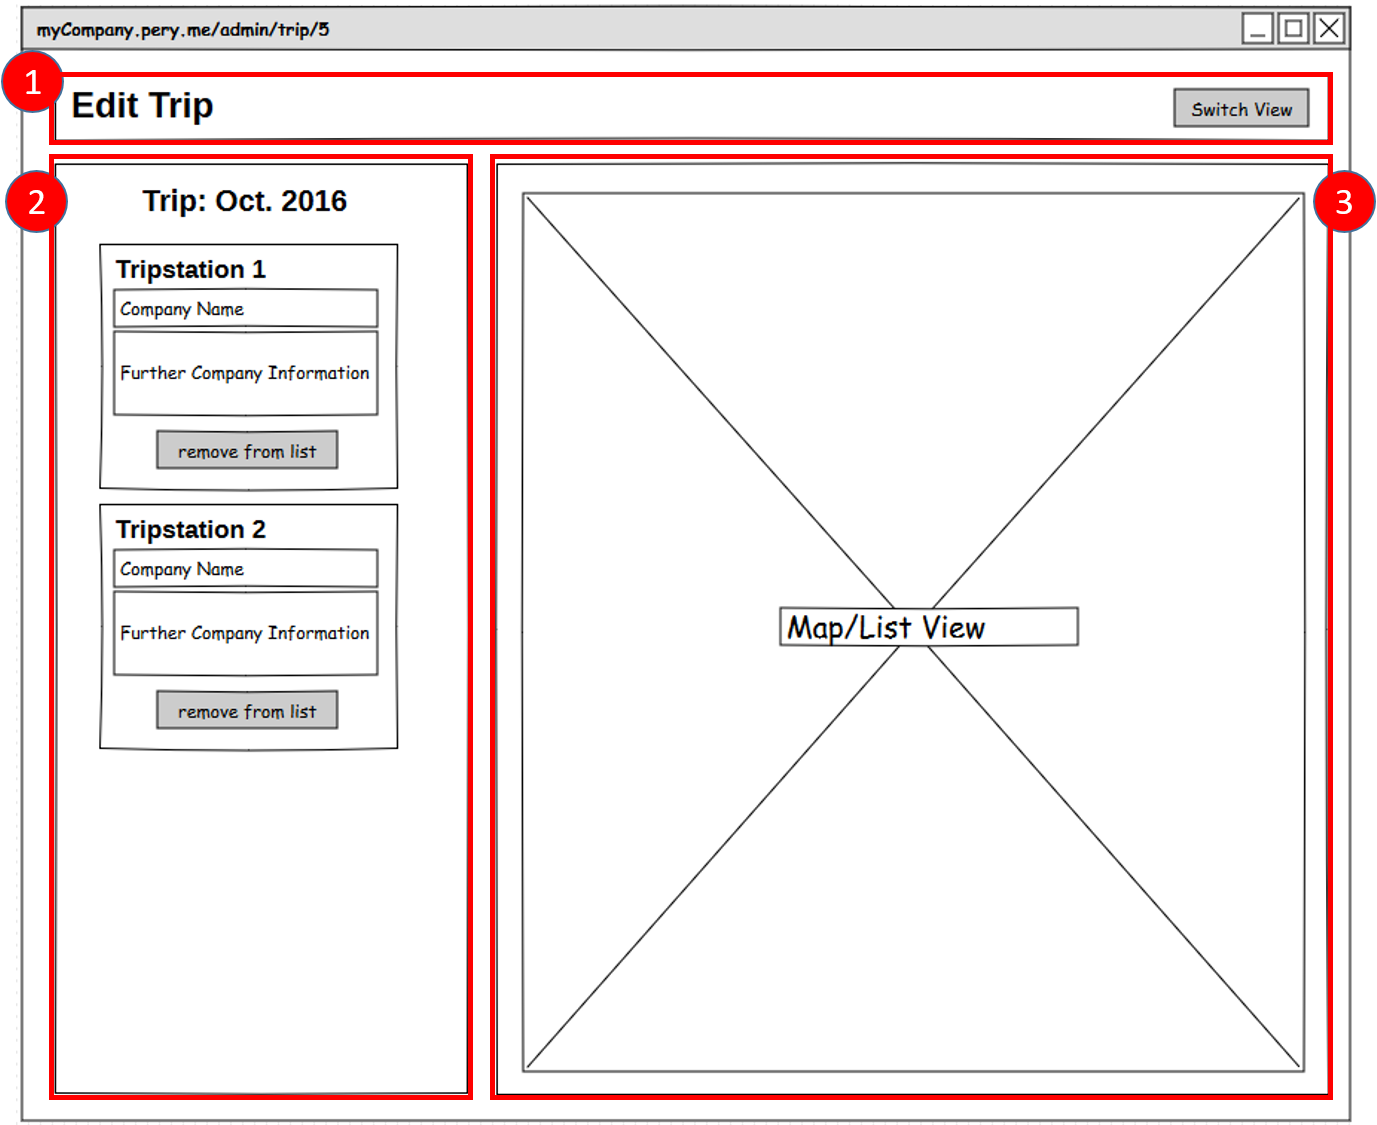
\includegraphics[width=0.8\linewidth]{img/Mockups/prototypMockup}
\caption[Mockup des Prototyps]{Mockup des Prototyps. Markierung 1: Kopfbereich, Markierung 2: Ergebnisse - Trip Liste, Markierung 3: Container für die umschaltbare Darstellung der Karten- und Listenansicht.}
\label{fig:prototypMockup}
\end{figure}


\end{document}
